\chapter{Generating random system properties}

One of the uses of random \gls{FOL} can be to generate random formula that represent system properties. That formula can be used as input for benchmark.

\section{Properties of computer systems}

System properties were first discussed in context of concurrency \cite{Lampert77} as a tool for formal verification multiprocess programs. One of first proposed properties were safety and liveness. These properties can apply to computer systems in general and be expressed in different formal systems.

\textbf{Liveness} \cite{Klimek99} is system property, that states, that something good will eventually happen.
Liveness formula guarantees that there is at least one case, where formula evaluates to true.

\textbf{Safety} \cite{Klimek99} is system property, that states, that something bad will never happens.
Safety formula must always be satisfied.

An informal example of system with liveness and safety properties could be an elevator. Statement: "Elevator will eventually stop" is liveness property of elevator as may be running now but eventually will hit the ceiling or floor. Statement: "Elevator must never run when the door is open" is safety property - the statement is always true.

\section{Properties of computer systems in first order logic}

In \gls{FOL} liveness and safety can be expressed as quantifiers, safety as universal quantifier and liveness as existential quantifier. 
If we were to use previously mentioned elevator example, the statements can be written as follows:

\begin{itemize}
  \item "Elevator will eventually stop" can be converted to logic formula: $\exists_t e(t)$ where predicate $e$ means "elevator is still", assuming $t<\infty$. The formula reads: there exists moment $t$ that the elevator is not moving
  \item "Elevator must never run when the door is open" can be converted to logic formula: $\forall_t \neg e(t) \land d(t)$ where predicate $e$ means "elevator is still" and $d$ means "doors are open". The formula reads: for every moment $t$ elevator is running and the doors are shut (at the same time).
\end{itemize}

\subsection{Properties of computer systems in first order logic in quantifier free}

Every \gls{FOL} can be converted to \gls{CNF}, so system properties can be also represented in \gls{CNF} but quantifiers must be also converted to CNF. The process of removing all the existential quantifiers from a formula is known as skolemization. The result is a formula in skolem normal form that is equivalent in computational complexity to the original. Skolemization follows several rules:


\begin{itemize}
  \item Variables bound by existential quantifiers which are not inside the scope of universal quantifiers can simply be replaced by constants - $\exists_t e(t)$ can be replaced by $e(f)$ where $f$ is new constant (functor)
  \item When the existential quantifier is inside a universal quantifier, the bound variable must be replaced by a Skolem function of the variables bound by universal quantifiers - $\forall_x  e(x) \land \exists_y e(t)$ can be replaced as $\forall_x e(x) \land e(f(x))$ 
\end{itemize}


Elevator example converted to quantifier free form looks as follows\footnote{removing quantifiers from first order logic can be automated with TPTP utility using TPTP2X utility, option \mintinline{text}{-t clausify}~\ref{sub:AdditionalToolsInTPTPLibrary} }::
\begin{itemize}
  \item "Elevator will eventually stop" $\exists_t e(t)$ in quantifier free form: $e(f)$ - new constant functor $f$ replaced variable $t$
  \item "Elevator must never run when the door is open" $\forall_t \neg e(t) \land d(t)$ in quantifier free form: $\neg e(X) \land d(Y)$ - 2 new variables $X$ and $Y$ replaced variable $t$ bounded to universal quantifier
\end{itemize}

In conclusion safety and liveness can be represented in CNF as 2 form of predicates: liveness as predicate, where arguments are only constant functors, safety as predicate where arguments are variables.

\section{Dataset with system properties}

The goal is to generate liveness and safety clauses, but do not mix them. In order to achieve that, class $PredicateGenerator$ needs to be modified to yield either formulas with all variables (safety) or formulas with 0-arity functor (liveness). To achieve that $PredicateGenerator$ was subclassed (see picture \ref{pic:SafetyLivenessGeneratorPreset}) and used to create alternative version of $CNFFormulaGenerator$. To control functors parameter $functor_arity$ needs to be set to allow only 0-arity functors, $FunctorGenerator$ subgenerator doe not need to be modified. Using newly defined $SafetyLivenessPredicateGenerator$ new preset is defined: $CNFSafetyLivenessGenerator$.

\begin{figure}[h]
\begin{centering}
  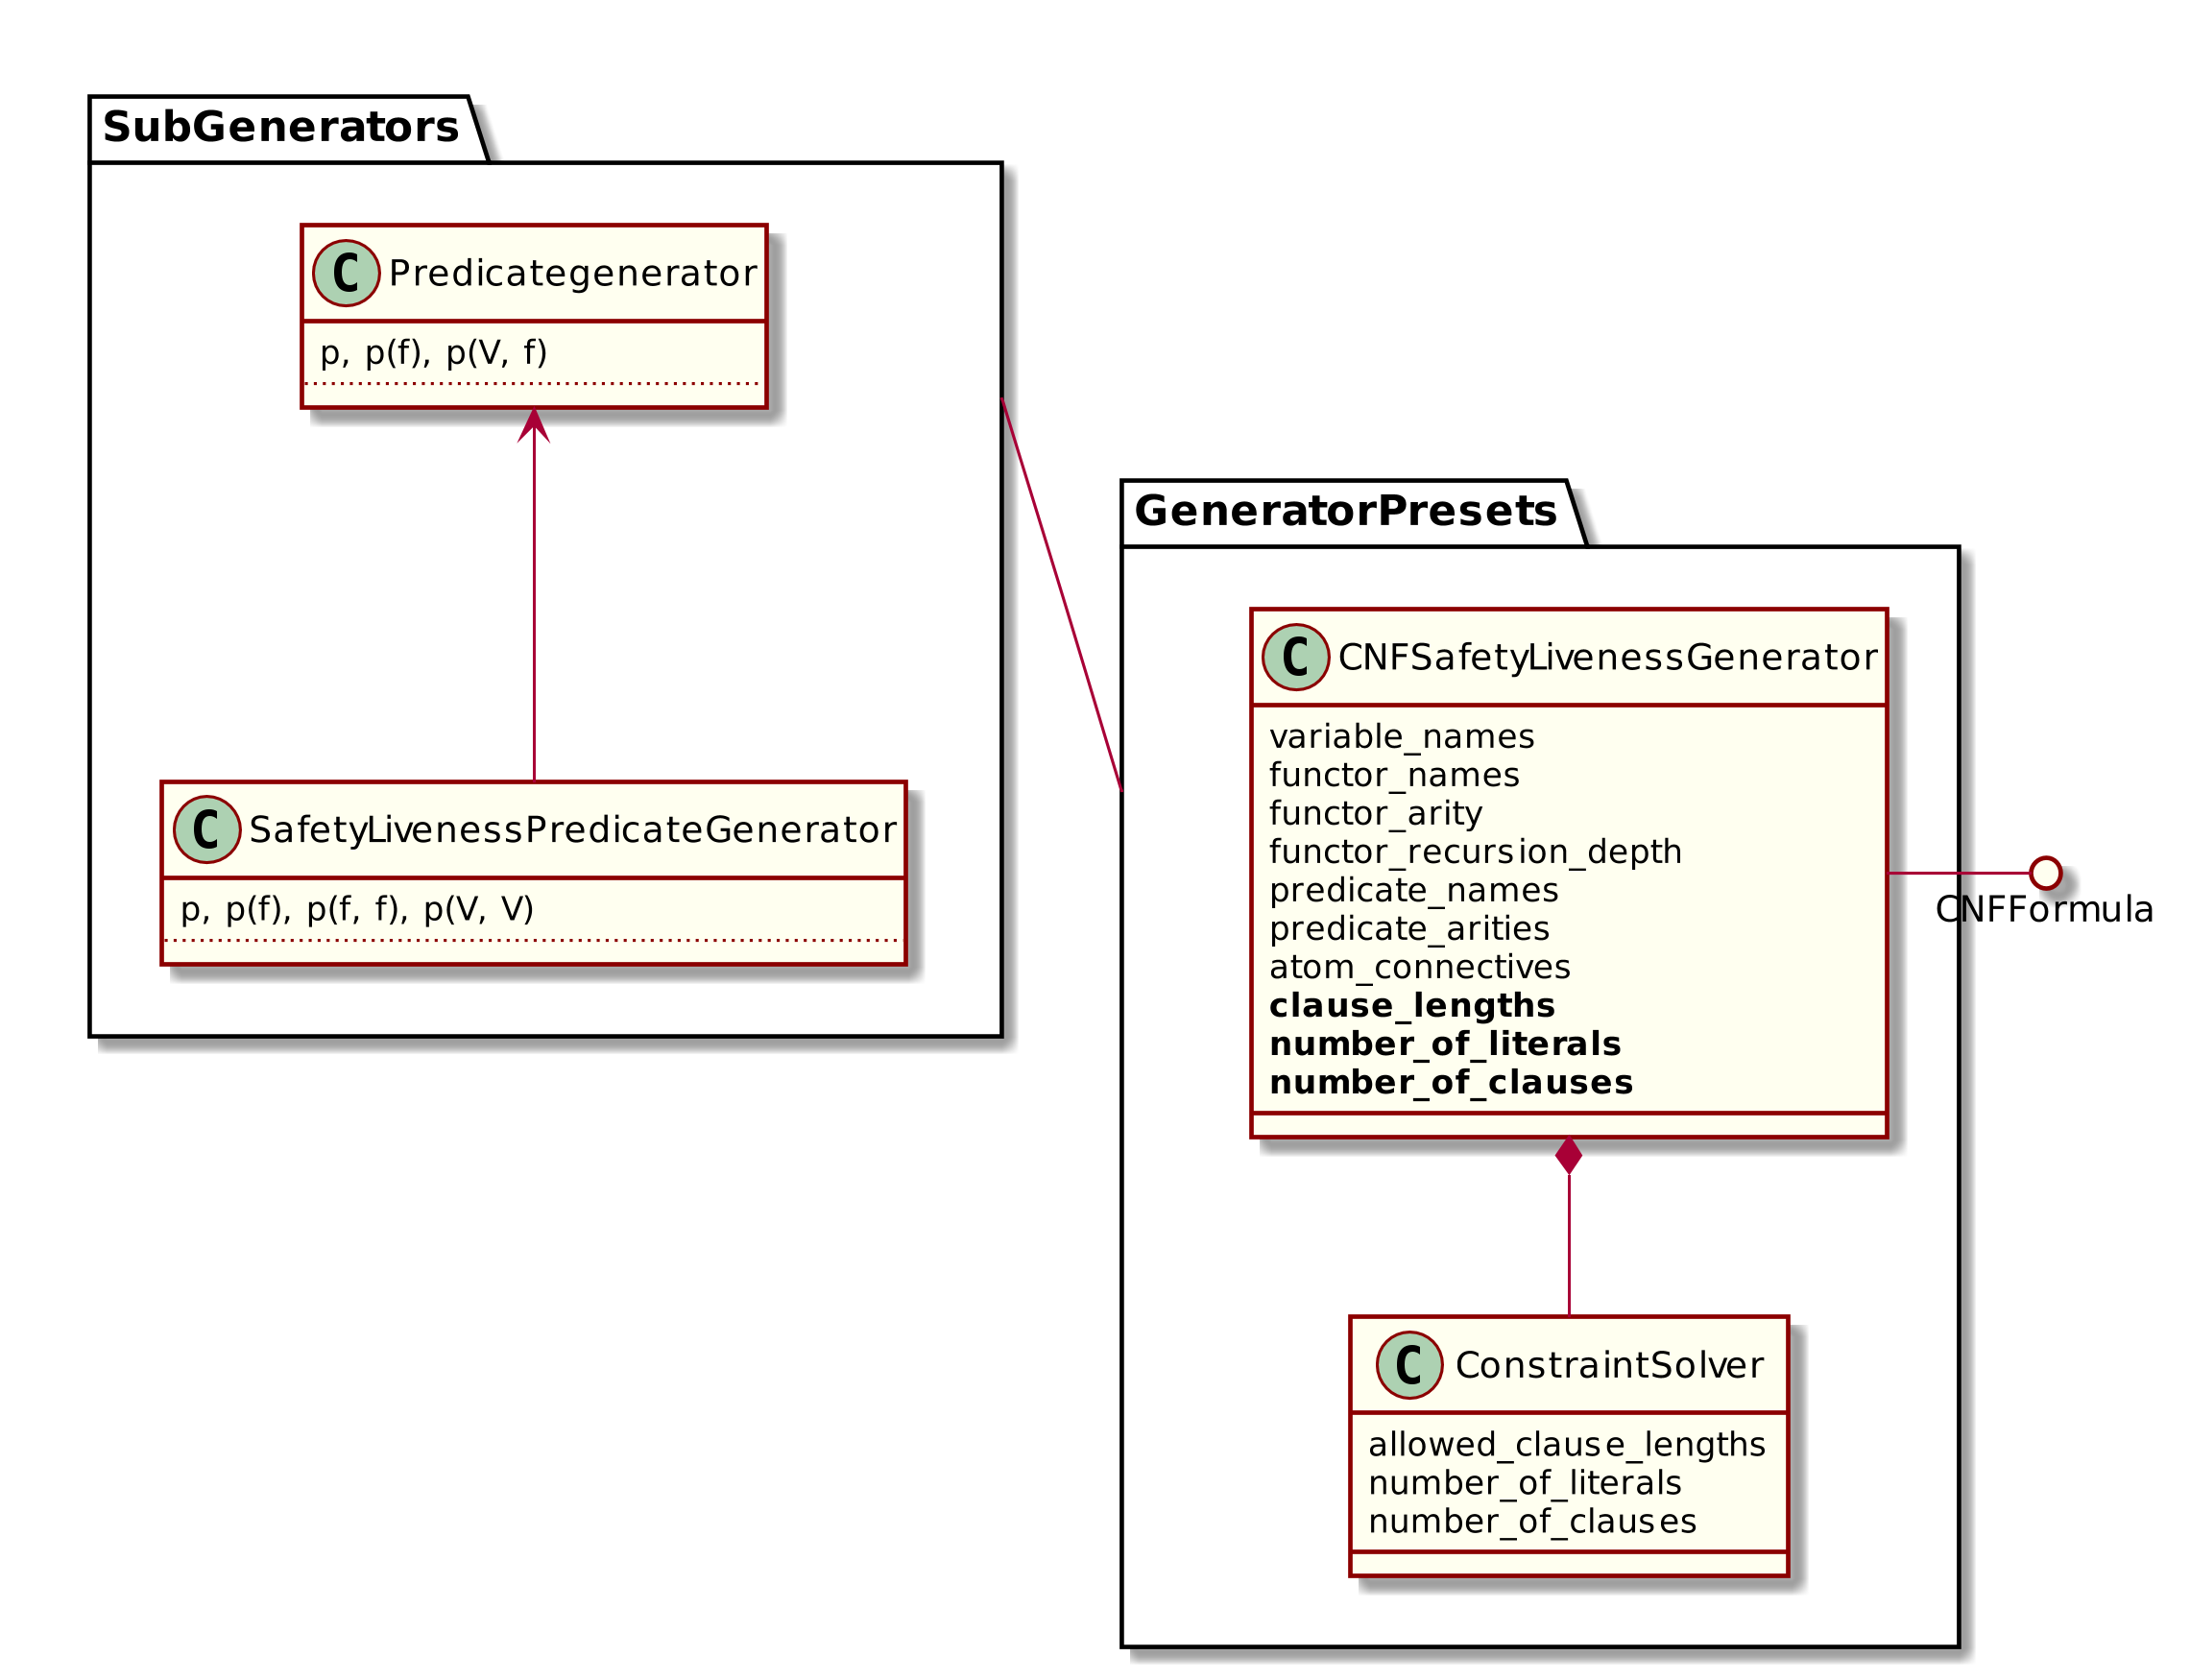
\includegraphics[width=\textwidth]{logic-formula-generator/fol/safety_liveness_predicate_generator.png}
  \caption{Subclassed PredicateGenerator mimics safety and liveness formulas}
  \label{pic:SafetyLivenessGeneratorPreset}
\end{centering}
\end{figure}

In this study the impact of ratio of number of atoms to number of clauses will be presented.
Formulas with 1000 atoms and 100, 200, 300, 400, 500 clauses were generated, 50 for each combination, 250 in total. 50 formulas is rather small sample to reason about, but it was chosen because of time and hardware limitations. Number of atoms and number of clauses can vary within 5\%, although solver tends to yield small numbers first in general. The rest of parameters for formulas is shown in listing~\ref{lis:CNFSafetyLivenesSnippet}.

\begin{listing}[ht]
  \caption{Snippet for generating dataset of safety and liveness formulas}
  \label{lis:CNFSafetyLivenesSnippet}
\begin{minted}{python}
gen = CNFSafetyLivenessGenerator(
    variable_names={f'V{i}' for i in range(10)},
    functor_names={f'f{i}' for i in range(20)}, functor_arity={0},
    functor_recursion_depth=0,
    predicate_names={f'p{i}' for i in range(20)}, predicate_arities={i for i in range(5)},
    atom_connectives={''},
    clause_lengths={i for i in range(2, 11)},
    number_of_clauses=IntegerRange.from_relative(number_of_clauses, threshold),
    number_of_literals=IntegerRange.from_relative(number_of_literals, threshold),
    literal_negation_chance=0.1,
)
\end{minted}
\end{listing}

\section{Results}

Formulas were generated and were benchmarked against solvers Prover9 and SPASS. Following charts present results in similar manner: on each chart there are 2 graphs: orange bar graph represents atom to clause ratio (2 means there are 2 atom for each clause) and blue scatter chart represents measured value: either time of execution (in seconds) or peak memory usage during execution. Maximum execution time of single formula was trimmed at 300 seconds (it remains unknown if formula is satisfiable or unsatisfiable). If execution time of formula is less than 300 seconds, it means it that solver concluded if formula is satisfiable or unsatisfiable, it is not relevant which one.

First thing worth noticing based on picture \ref{pic:Prover9NumberOfClausesVsTime} and \ref{pic:SPASSNumberOfClausesVsTime} is SPASS solver is capable of solving much more formulas than Prover9. SPASS returned only 5 timeouts which compared to Prover9 56 timeouts out of 250 test cases works to the advantage of SPASS over Prover9 in tested area. This difference is beyond measurement error even though generated formulas are random. 

SPASS to a certain extent uses constant memory (picture \ref{pic:SPASSNumberOfClausesVsMemory}) whereas Prover9 (picture \ref{pic:Prover9NumberOfClausesVsMemory}) requires notably more memory the longer it runs. Memory range used by SPASS varies between 56 Mb and 83 Mb, whereas Prover9 uses much wider range of memory - between 2 Mb up to 555 Mb.

The most important observation based on picture \ref{pic:Prover9NumberOfClausesVsTime} and \ref{pic:SPASSNumberOfClausesVsTime} is the higher the atoms/clauses ratio the longer the time of execution is thus timeouts are more frequent. The turning point of this observation seems to occur around atoms/clauses ratio equal to 5, at least for Prover9, as at this point more and more timeouts happen. This observation for SPASS might not so viable as this there are only 5 timeouts and the rest of formulas were computed in similar time (243 formulas in less than 1 second) therefore result can be considered a coincidence as dataset is random. We can get more hints of the same conclusion for SPASS as we have for Prover9 from memory charts in picture \ref{pic:SPASSNumberOfClausesVsMemory} where visibly for higher atoms/clauses ratio more than average of 60 Mb of memory is used, and for the lower ratio memory usage drops slightly below the average.

The range of number of atoms was specified in input parameters for generator and is presented in picture \ref{pic:Prover9NumberOfAtomsVsTime} and \ref{pic:Prover9NumberOfAtomsVsTimeSortedByAtoms}. The influence of number of atoms threshold of 5\% is insignificant to the influence of atoms/clauses ratio.

\begin{figure}[h]
  \centering
  \includegraphics[width=0.8\textwidth]{"logic-formula-generator/dataset_analysis/cnf charts/01 Prover9 number of clauses vs time".jpg}
  \caption{Prover9 number of clauses vs time, formulas are sorted by number of clauses}
  \label{pic:Prover9NumberOfClausesVsTime}
\end{figure}

\begin{figure}[h]
  \centering
  \includegraphics[width=0.8\textwidth]{"logic-formula-generator/dataset_analysis/cnf charts/11 SPASS number of clauses vs time".jpg}
  \caption{SPASS number of clauses vs time, formulas are sorted by number of clauses}
  \label{pic:SPASSNumberOfClausesVsTime}
\end{figure}

\begin{figure}[h]
  \centering
  \includegraphics[width=0.7\textwidth]{"logic-formula-generator/dataset_analysis/cnf charts/02 Prover9 number of clauses vs peak memory".jpg}
  \caption{Prover9 number of clauses vs peak memory, formulas are sorted by number of clauses}
  \label{pic:Prover9NumberOfClausesVsMemory}
\end{figure}

\begin{figure}[h]
  \centering
  \includegraphics[width=0.7\textwidth]{"logic-formula-generator/dataset_analysis/cnf charts/12 SPASS number of clauses vs peak memory".jpg}
  \caption{SPASS number of clauses vs peak memory, formulas are sorted by number of clauses}
  \label{pic:SPASSNumberOfClausesVsMemory}
\end{figure}

\begin{figure}[h]
  \centering
  \includegraphics[width=0.7\textwidth]{"logic-formula-generator/dataset_analysis/cnf charts/03 Prover9 number of atoms vs time".jpg}
  \caption{Prover9 number of atoms vs time of execution, formulas are sorted by number of clauses}
  \label{pic:Prover9NumberOfAtomsVsTime}
\end{figure}

\begin{figure}[h]
  \centering
  \includegraphics[width=0.7\textwidth]{"logic-formula-generator/dataset_analysis/cnf charts/03 Prover9 number of atoms vs time sorted by atoms".jpg}
  \caption{Prover9 number of atoms vs time of execution, formulas are sorted by number of atoms}
  \label{pic:Prover9NumberOfAtomsVsTimeSortedByAtoms}
\end{figure}
